\documentclass[12pt]{article}

\usepackage{fullpage}
\usepackage{multicol,multirow}
\usepackage{tabularx}
\usepackage{ulem}
\usepackage{graphicx}%Вставка картинок правильная
\usepackage{float}%"Плавающие" картинки
\usepackage{wrapfig}%Обтекание фигур (таблиц, картинок и прочего)
\usepackage[utf8]{inputenc}
\usepackage[russian]{babel}

% Оригиналный шаблон: http://k806.ru/dalabs/da-report-template-2012.tex

\begin{document}

\section*{Лабораторная работа №\,5 по курсу дискрeтного анализа: суффиксные деревья}

Выполнил студент группы 08-307 МАИ \textit{Дегтярев Денис Андреевич}.

\subsection*{Условие}

Найти образец в тексте используя статистику совпадений.

\subsection*{Формат ввода}

На первой строке располагается образец, на второй — текст.

\subsection*{Формат вывода}

Последовательность строк содержащих в себе номера позиций, начиная с которых встретился образец. Строки должны быть отсортированы в порядке возрастания номеров.

\subsection*{Метод решения}

Находим образец подстроки в тексте с помощью статистики совпадений

\subsection*{Описание программы}

Строим суффиксное дерево по паттерну. Затем вызываем метод GetMatchStatistics для того, чтобы построить статистику для вершин. Если данная статистика равна размеру паттерна, значит выводим индекс данной статистики(соответствует букве).

\subsection*{Дневник отладки}  
  
Все прошло с первого раза(удивлен)

\subsection*{Тест производительности}

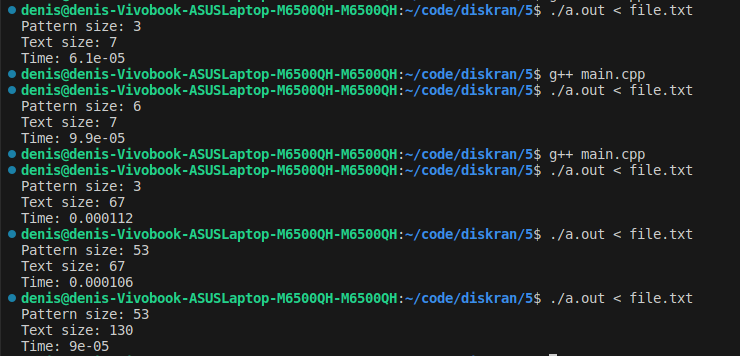
\includegraphics[width=7in]{time.png}

\subsection*{Недочёты}

Возможно, можно еще оптимизирвоать по скорости и убрать пару ненужного кода

\subsection*{Выводы}

Выполнив лабораторную работу №5 по курсу «Дискретный анализ», я изучил
различные методы построения суффиксных деревьев и алгоритмы, работающие с помощью суффиксных деревьев, и убедился, что они помогают в оптимизации
решений различных задач, связанных с поиском подстроки в строке, благодаря представления текста в более компактном виде.

\end{document}
